\documentclass[10pt]{beamer}
\usetheme{Madrid}
\usepackage[T2A]{fontenc}
\usepackage[utf8]{inputenc}
\usepackage[russian]{babel}
\usepackage{amsmath}
\usepackage{amsfonts}
\usepackage{amssymb}
\usepackage{comment}
\usepackage[all]{xy}

%\newtheorem{theorem}{Теорема}

\author{Баев А.Ж.}
\title{Введение в численные методы. \\ Точные методы решения СЛАУ}
\institute{Казахстанский филиал МГУ} 
\date{09 февраля 2019}
%\subject{} 

\usepackage{tikz}
\usetikzlibrary{patterns} 
\usetikzlibrary{arrows, matrix, positioning, decorations.pathreplacing}

\usepackage{listings}
\lstset{language=python}
\lstset{basicstyle=\ttfamily}  
\lstset{keywordstyle=\color{blue}}
\lstset{frame=single}
\lstset{numbers=left}
\lstset{tabsize=4}



\usepackage{graphicx}

\begin{document}

\maketitle


\begin{frame}[fragile]
\frametitle{План на семестр}

\begin{enumerate}
\item СЛАУ (точные методы)
\item СЛАУ (итерационные методы)
\item решение нелинейных уравнений
\item интерполяция 
\item аппроксимация
\item интегрирование
\item дифференцирование
\end{enumerate}

\end{frame}


\begin{frame}[fragile]
\frametitle{Линейная алгебра}

Решение системы линейных алгебраических уравнений:

$$A x = f$$

где $A \in \mathbb{R}^{n \times n}$, $x \in \mathbb{R}^{n}$, $f \in \mathbb{R}^{n}$.

Дано $A$, $f$. Найти $x$.

\end{frame}


\begin{frame}[fragile]
\frametitle{Метод прогонки}

Метод прогонки (англ. tridiagonal matrix algorithm) 

Алгоритм Томаса (англ. Thomas algorithm)

Дана квадратная трехдиагональная матрица $A \in \mathbb{R}^{n \times n}$. 

Решить СЛАУ $A x = f$.

$$
\begin{pmatrix}
b_1&c_1& 0 & 0 &\hdots&  & 0 & 0 & 0\\
a_2&b_2&c_2& 0 &\hdots&  & 0 & 0 & 0\\
0 &a_3&b_3&c_3&\hdots&  & 0 & 0 & 0\\
0 & 0 &a_4&b_4&\hdots&  & 0 & 0 & 0\\
\vdots&\vdots&\vdots&\vdots&\ddots&  &\vdots&\vdots&\vdots\\
0 & 0 & 0 & 0 &\hdots&  &b_{n-2}&c_{n-2}& 0\\
0 & 0 & 0 & 0 &\hdots&  &a_{n-1}&b_{n-1}&c_{n-1}\\
0 & 0 & 0 & 0 &\hdots&  & 0 &a_{n}&b_{n}\\
\end{pmatrix}
\begin{pmatrix}
x_1\\
x_2\\
x_3\\
x_4\\
\vdots\\
x_{n-2}\\
x_{n-1}\\
x_n\\
\end{pmatrix}
=
\begin{pmatrix}
f_1\\
f_2\\
f_3\\
f_4\\
\vdots\\
f_{n-2}\\
f_{n-1}\\
f_n\\
\end{pmatrix}
$$
\end{frame}


\begin{frame}[fragile]
\frametitle{Метод прогонки}

В виде строчных соотношений:
$$
\begin{cases}
b_1 x_1 + c_1 x_{2}                 &= f_1\\
a_i x_{i-1} + b_i x_i + c_i x_{i+1} &= f_i, i = 2,..., n-1\\
a_n x_{n-1} + b_n x_n               &= f_n
\end{cases}
$$
\end{frame}


\begin{frame}[fragile]
\frametitle{Метод прогонки}
1) Добавим фиктивные элементы: $a_1 = c_n = 0$. 

Добавим фиктивные решения: $x_0 = x_{n+1} = 0$.

\begin{equation}
\label{sweeptask}
a_i x_{i-1} + b_i x_i + c_i x_{i+1} = f_i, i = 1,..., n
\end{equation}

\end{frame}


\begin{frame}[fragile]
\frametitle{Метод прогонки}
2) Допустим $x_i$ выражаются линейно друг через друга :
\begin{equation}
\label{sweepidea}
x_{i-1} = \alpha_i x_i + \beta_i, i = 1, ..., n+1
\end{equation}

Подставим (\ref{sweepidea}) в соотношение (\ref{sweeptask}) при $i = 1, ...,  n$:
$$ a_i  ( \alpha_i x_i + \beta_i ) + b_i x_i + c_i x_{i+1} = f_i$$
$$ (a_i  \alpha_i + b_i) x_i + c_i x_{i+1} = f_i - a_i \beta_i$$
$$ x_i = \frac{- c_i}{a_i  \alpha_i + b_i} x_{i+1} + \frac{f_i - a_i \beta_i}{a_i  \alpha_i + b_i}$$
\end{frame}


\begin{frame}[fragile]
\frametitle{Метод прогонки}
3) Из предположения, что $x_{i} = \alpha_{i+1} x_{i+1} + \beta_{i+1}, i = 0, ..., n
$:
$$
\begin{cases}
\alpha_{i+1} = \frac{- c_i}{a_i  \alpha_i + b_i} \\
\beta_{i+1} = \frac{f_i - a_i \beta_i}{a_i  \alpha_i + b_i}
\end{cases}
i = 1, ..., n
$$

С учетом того, что $x_0 = 0$ получаем $\alpha_1 = \beta_1 = 0$.
\end{frame}


\begin{frame}[fragile]
\frametitle{Метод прогонки}
Прямой ход прогонки:
\begin{equation}
\label{sweepfor}
\begin{cases}
\alpha_1 = 0, \beta_1 = 0,\\
\alpha_{i+1} = \frac{- c_i}{a_i  \alpha_i + b_i}\\
\beta_{i+1} = \frac{f_i - a_i \beta_i}{a_i  \alpha_i + b_i}\\
\end{cases}
i = 1, ..., n
\end{equation}

Схема вычисления:
\begin{displaymath} 
\xymatrix{
\alpha_1 = 0 \ar[r] \ar[rd] & \alpha_2 \ar[r] \ar[rd] & \alpha_3 \ar[r] \ar[rd] & ... \ar[r] \ar[rd]  & 
\alpha_n \ar[r] \ar[rd]     & \alpha_{n+1}	\\ 
\beta_1 = 0 \ar[r]          & \beta_2 \ar[r]          & \beta_3 \ar[r]          & ... \ar[r]          & 
\beta_n \ar[r]              &  \beta_{n+1}	\\ 
}
\end{displaymath}
\end{frame}


\begin{frame}[fragile]
\frametitle{Метод прогонки}
Обратный ход прогонки:
\begin{equation}
\label{sweepback}
\begin{cases}
x_{n+1} &= 0\\
x_{i} &= \alpha_{i+1} x_{i+1} + \beta_{i+1}, i = \overline{n,1}
\end{cases}
\end{equation}

Схема вычисления:
\begin{displaymath} 
\xymatrix{
\alpha_1 	& \alpha_2 \ar[ld] 	& \alpha_3 \ar[ld]	& ... \ar[ld]	& \alpha_{n-1} \ar[ld] 	& \alpha_n \ar[ld]	& \alpha_{n+1}	\ar[ld]\\ 
x_1 		& x_2 \ar[l]   		& x_3 \ar[l] 		& ... \ar[l] 	& x_{n-1} \ar[l]		& x_n \ar[l] 		&  x_{n+1} = 0 \ar[l]\\
\beta_1 	& \beta_2 \ar[ul] 	& \beta_3 \ar[ul]	& ... \ar[ul]	& \beta_{n-1} \ar[ul]	& \beta_n \ar[ul]	&  \beta_{n+1} \ar[ul]	\\
}
\end{displaymath}

\end{frame}


\begin{frame}[fragile]
\frametitle{Метод прогонки (пример)}

$$
\begin{pmatrix}
4&3&0 \\
1&3&1 \\
0&1&2 \\
\end{pmatrix}
\begin{pmatrix}
x_1\\
x_2\\
x_3\\
\end{pmatrix}
=
\begin{pmatrix}
10\\
10\\
8\\
\end{pmatrix}
$$

Запишем вектора $a$, $b$, $c$ и $f$:
$$a = (0, 1, 1)$$
$$b = (4, 3, 2)$$
$$c = (3, 1, 0)$$
$$f = (10, 10, 8)$$

\end{frame}


\begin{frame}[fragile]
\frametitle{Метод прогонки (пример)}

1) Вычислим коэффициенты $\alpha$ и $\beta$ прямым ходом прогонки (\ref{sweepfor}):

\begin{tabular}{ll}
$\alpha_1 = 0$ & $\beta_1 = 0$ 
\\

$\alpha_2 = \frac{- c_1}{a_1  \alpha_1 + b_1} = \frac{-3}{0 \cdot 0 + 4} = - \frac{3}{4}$ & 
$\beta_2 = \frac{f_1 - a_1 \beta_1}{a_1 \alpha_1 + b_1} = \frac{10 - 0 \cdot 0}{0 \cdot 0 + 4} = \frac{5}{2}$ 
\\

$\alpha_3 = \frac{- c_2}{a_2  \alpha_2 + b_2} = \frac{-1}{1 \cdot (- \frac{3}{4}) + 3} = - \frac{4}{9}$ &
$\beta_3 = \frac{f_2 - a_2 \beta_2}{a_2 \alpha_2 + b_2} = \frac{10 - 1 \cdot \frac{5}{2}}{1 \cdot (- \frac{3}{4}) + 3} = \frac{10}{3}$ \\

$\alpha_4 = \frac{- c_3}{a_3  \alpha_3 + b_3} = \frac{0}{1 \cdot (-\frac{4}{9}) + 2} = 0$ & 
$\beta_4 = \frac{f_3 - a_3 \beta_3}{a_3 \alpha_3 + b_3} = \frac{8 - 1 \cdot \frac{10}{3}}{1 \cdot (-\frac{4}{9}) + 2} = 3$
\\
\end{tabular}


2) Вычислим решение $x$ обратным ходом прогонки (\ref{sweepback}):

$x_4 = 0$

$x_3 = \alpha_4 x_4 + \beta_4 = 0 * 0 + 3 = 3$

$x_2 = \alpha_3 x_3 + \beta_3 = - \frac{4}{9} * 3 + \frac{10}{3} = 2$

$x_1 = \alpha_2 x_2 + \beta_2= - \frac{3}{4} * 2 + \frac{5}{2} = 1$

Ответ: $x = (1, 2, 3)$.

\end{frame}


\begin{frame}[fragile]
\frametitle{Метод прогонки (реализация)}

\begin{lstlisting}
sweep(a[1:n], b[1:n], c[1:n], f[1:n]) -> x[1:n]
	alpha[1:n+1]
	beta[1:n+1]

	a[1] := 0
	c[n] := 0
	alpha[1] := 0
	beta[1] := 0
	for i := 1 .. n
    	d := a[i] * alpha[i] + b[i]
    	alpha[i+1] := - c[i] / d
    	beta[i+1] := (f[i] - a[i] * beta[i]) / d

	x[n+1] := 0
	for i := n .. 1
    	x[i] := alpha[i+1] * x[i+1] + beta[i+1]

    return x[1:n]
\end{lstlisting}

\end{frame}


\begin{frame}[fragile]
\frametitle{Метод прогонки (реализация)}
\begin{lstlisting}
sweep(a[1:n], b[1:n], c[1:n], f[1:n]) -> x[1:n]
	alpha[1:n+1]
	beta[1:n+1]

	a[1] := 0
	c[n] := 0
	alpha[1] := 0
	beta[1] := 0
	for i := 1 .. n
    	d := a[i] * alpha[i] + b[i]
    	alpha[i+1] := - c[i] / d
    	beta[i+1] := (f[i] - a[i] * beta[i]) / d

	x[n] := beta[n+1]
	for i := n-1 .. 1
    	x[i] := alpha[i+1] * x[i+1] + beta[i+1]

    return x
\end{lstlisting}
\end{frame}

\begin{frame}[fragile]
\frametitle{Метод прогонки (алгоритмическая сложность)}

\begin{enumerate}
\item Прямой ход --- $f(n) = 4n$;
\item Обратный ход --- $f(n) = n$;
\item Итог --- $f(n) = 5n$.
\end{enumerate}

Асимптотика прямого и обратного хода: $\Theta(n)$.

\end{frame}

\begin{frame}[fragile]
\frametitle{Метод прогонки (существование решения)}
Будем говорить, что матрица имеет \textbf{диагональное преобладание}, если

$$ |a_{ii}| > \sum_{i\neq j}|a_{ij}|$$

Для матриц с диагональным преобладанием справедливо утверждение, что все главные миноры отличны от нуля и система уравнений имеет единственное решение.
\end{frame}

\begin{frame}[fragile]
\frametitle{Метод прогонки (устойчивость решения)}
Если матрица обладает диагональным преобладанием, то
$$ |\alpha_{i}| < 1$$

Доказательство:
$$|\alpha_{i+1}| = \left|\frac{b_i}{a_i \alpha_i + c_i}\right| \leqslant \frac{|b_i|}{|c_i| - |a_i|} < 1 $$

Это означает, что ошибка $x_{i+1} = \alpha_i x_i + \beta_i$ не превышает ошибки в $x_i$.
\end{frame}

\begin{frame}[fragile]
\frametitle{Метод Холецкого}

Пусть $A = A^{T}$ и $A > 0$. Тогда
$$ A = S^T S$$
где $S$ --- верхнетреугольная матрица.

\vfill

Решение $Ax = f$ сводится к решению $S^{T} y = f$ и $S x = y$.
\end{frame}

\begin{frame}[fragile]
\frametitle{Метод Холецкого}

$$a_{i j} = \sum_{k=1}^{i} s_{ki} s_{kj}, j \geqslant i$$.

Получаем:
$$s_{i i} = \sqrt{a_{ii} - \sum_{k=1}^{i-1} s_{ki}^2}, j = i + 1 ... n$$
$$s_{i j} = \frac{a_{ij} - \sum_{k=1}^{i-1} s_{ki} s_{kj}}{s_{ii}}, j = i + 1 ... n$$

Зачем?
\end{frame}

\begin{frame}[fragile]
\frametitle{Обусловленность систем (норма вектора)}

Введем норму вектора $||x||$:

\begin{enumerate}
\item $||x|| = 0 \Leftrightarrow x = 0$.
\item $||x + y|| \leqslant ||x|| + ||y||$
\item $ \alpha \in \mathbb{R}$ $||\alpha x|| = |\alpha| ||x||$.
\end{enumerate}

Например:
\begin{enumerate}
\item $||x||_1 = |x_1| + |x_2| + \ldots + |x_n|$.
\item $||x||_2 = \sqrt{x_1^2 + x_2^2 + \ldots + x_n^2}$.
\item $||x||_{\infty} = \max_i |x_i|$.
\end{enumerate}
\end{frame}

\begin{frame}[fragile]
\frametitle{Обусловленность систем (норма матрицы)}

Матричная норма $||A||$ согласуется нормой вектора $||x||$:

$$ 
||A|| = \sup_{x \neq 0} \frac{||Ax||}{||x||}
$$

Например:
\begin{enumerate}
\item $||A||_1 = \max_i \left( \sum_j |a_{ i j }| \right)$.
\item $||A||_2 = \max_i |\lambda_i|$.
\item $||A||_{\infty} = \max_j \left( \sum_i |a_{ i j }| \right)$.
\end{enumerate}
\end{frame}

\begin{frame}[fragile]
\frametitle{Обусловленность систем (основное неравенство)}

$$ 
||A x|| \leqslant ||A|| ||x||
$$
\end{frame}


\begin{frame}[fragile]
\frametitle{Обусловленность систем}

Решаем $Ax = f$.

Как сильно может измениться решение $x$ в результате изменения правой части $f$?

\end{frame}


\begin{frame}[fragile]
\frametitle{Обусловленность систем}

$$\delta x = x - \tilde{x}$$
$$\delta f = f - \tilde{f}$$

Получаем
$$A ( \delta x ) = \delta f $$

Выпишем два неравенства
$$|| \delta x || = || A^{-1} ( \delta f )|| \leqslant ||A^{-1}|| \cdot ||\delta f||$$
$$|| f || = || A x|| \leqslant ||A|| \cdot ||x||$$

Перемножим
$$|| \delta x || \cdot || f || \leqslant ||A|| \cdot ||A^{-1}|| \cdot ||\delta f|| \cdot ||x||$$

$$\frac{|| \delta x ||}{||x||} \leqslant ||A|| \cdot ||A^{-1}|| \cdot \frac{||\delta f||}{||f||}$$

\end{frame}

\begin{frame}[fragile]
\frametitle{Обусловленность систем}

Чем меньше число обусловленности, тем лучше:
$$\mu = ||A|| \cdot ||A^{-1}|| $$

Пример матрицы с хорошим число обусловленности
$$
\begin{pmatrix}
10 & 0 \\
0 & 11 \\
\end{pmatrix}
$$

Пример матрицы с плохим числом обусловленности
$$
\begin{pmatrix}
10 & 10 \\
10 & 11 \\
\end{pmatrix}
$$

\end{frame}

\begin{frame}[fragile]
\frametitle{Обусловленность систем}

\begin{lstlisting}
import numpy as np
 
a = np.array([[10, 10], [10, 11]])
b = np.linalg.inv(a)

mu = np.linalg.norm(a) * np.linalg.norm(b)
print(mu)
\end{lstlisting}

Вывод: 42.1000
\end{frame}

\begin{frame}[fragile]
\frametitle{Обусловленность систем}

\begin{lstlisting}
import numpy as np
 
a = np.array([[10, 10], [10, 11]])

mu = np.linalg.cond(a)
print(mu)
\end{lstlisting}

Вывод: 42.0762
\end{frame}

\begin{frame}[fragile]
\frametitle{Метод прогонки}

\begin{lstlisting}
import scipy.linalg as sl

A = [ [0, 3, 1],
      [4, 3, 2],
      [1, 1, 0] ]
f = [10, 10, 8]
x = sl.solve_banded((1, 1), A, f)
print(x)
\end{lstlisting}

Вывод: [1, 2, 3]
\end{frame}

\begin{frame}[fragile]
\frametitle{Метод прогонки}

\begin{lstlisting}
import scipy.linalg as sl

A = [ [0, 3, 1],
      [4, 3, 2],
      [1, 1, 0] ]
f = [10, 10, 8]
x = sl.solve_banded((1, 1), A, f)
print(x)
\end{lstlisting}

Вывод: [1, 2, 3]
\end{frame}

\begin{frame}[fragile]
\frametitle{Разложение Холецкого}
\begin{lstlisting}
import numpy as np
import scipy.linalg as sl

L = np.array([ [1, 0, 0],
             [2, 1, 0],
             [3, 2, 1] ])
A = L.dot(np.transpose(L))
print(A)

L = sl.cholesky(A, lower=True)
print(L)
\end{lstlisting}
\end{frame}

\begin{frame}[fragile]
\frametitle{Упражнения}

1. Описать как связаны коэффициенты $\alpha_{i}$ и $\beta_{i}$ с матрицами в $LU$---разложении.

2. Докажите, что у матрицы с диагональным преобладанием все угловые миноры ненулевые.

3. Описать метод прогонки для блочно трёхдиагональная матрицы, в которой вместо элементов $a_i$, $b_i$, $c_i$ находятся подматрицы размера $k \times k$, а вместо $f_i$ --- вектор столбец размера $k$. Основная идея: $x_{i-1} = \alpha_i x_i + \beta_i$, где $\alpha_i \in \mathbb{R}^{k \times k}$, $\beta_i \in \mathbb{R}^k$.

\end{frame}

\begin{frame}[fragile]
\frametitle{Графики}

\begin{lstlisting}
import matplotlib.pyplot as plt
y = [1, 5, 2, 4, 3]
plt.plot(y)
plt.show()
\end{lstlisting}

\begin{center}
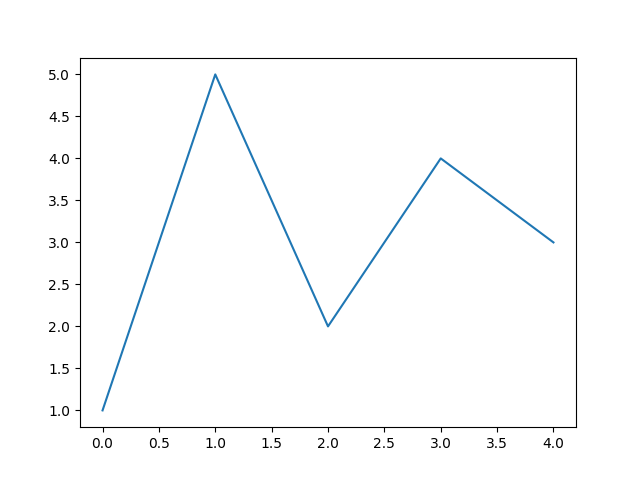
\includegraphics[scale=0.5]{matplotlib.png}
\end{center}
\end{frame}


\begin{frame}[fragile]
\frametitle{Домашнее задание №1}

\begin{enumerate}
\item Сравнить решение СЛАУ методом Гаусса на встроенной функции и  на своей реализации на случайной матрицей с диагональным преобладанием размером $100 \times 100$, $200 \times 200$ и т.д. Провести несколько экспериментов, пока время счёта меньше 1 сек. Построить графики зависимостей.

\item Сравнить решение СЛАУ методом Холецкого на встроенной функции и  на своей реализации на случайной положительно определённой матрицей с диагональным преобладанием размером $100 \times 100$, $200 \times 200$ и т.д. Провести несколько экспериментов, пока время счёта меньше 1 сек. Построить графики зависимостей.

\item Сравнить решение СЛАУ методом прогонки на встроенной функции и  на своей реализации на случайной трехдиагональной матрице с диагональным преобладанием размером $1000 \times 1000$, $2000 \times 2000$ и т.д. Провести несколько экспериментов, пока время счёта меньше 1 сек. Построить графики зависимостей.
\end{enumerate}

\end{frame}
\end{document}
